\chapter{Theoretical background}
This chapter gives a brief overview over the most important distributions and transformations that are used for the SimpleSTORM algorithm and the Colorcomposer. Also an introduction to the most important parts of a regular Charge-coupled Device (CCD) cameras is given as well as a section about the data the algorithm is designed for. 

\section{The data}
\subsection{Labeling}
The concept of direct stochastic optical reconstruction microscopy (dSTORM) \cite{heilemann} is, to label structures of interest with fluorophors that can be exited using a laser with the appropriate wavelength directly, in contrast to STORM techniques which need an additional activator fluorophore. A short time after the activation the fluorophors emit a photon and fall back to the unexited state or lose the ability to get exited, they bleach out. Special fluorophores have to be used that have a low probability to get activated. The result of this is that each fluorophore is visible only every thousandth frame or less often.\newline
The technique to stain the samples that was used for all real-world images in this thesis is called immunofluorescence. For this technique antibodies are used to attach the fluorescenic molecules to the samples. Antibodies target specific biomolecules within a cell that show their antigen. There are two classes of immunofluorescence techniques.\newline
Primary immunofluorescence uses only one antibody to that the fluorophore is directly attached.\newline
For secundary immunofluorescence two kinds of antibodies are used. One primary antibody that binds to the molecule or structure of interest and a second antibody that binds to the primary and carries the fluorophore.

\subsection{Description of the data sets}
The datasets for dSTORM microscopy that we recieve from our collaborators from
Bioquant are big datasets of several gigabyte in the Andor ".sif" format. Each
file conains a stack of pictures, normaly between 1000 and 10000, taken
consecutively with a fixed exposure time normally between 20 and 200 milliseconds. From now on the first two dimensions are called spatial dimensions. It is refered to third dimension of the data that results from the consecutive capturing of the images as temporal dimension.\newline

Figure \ref{rawStorm} shows a typical frame of raw data. In each frame there might be multiple fluorophores visible at the same time. Due to the large magnification, beyond the diffraction limit, the almost pointlike fluorophores appear as approximatly Gaussian shaped signals, their point spread functions. The fluorophores are either attached to the biological structures that are of interest or they form a cluster, called a bead.\newline

Beads are larger and brighter than spots from only one fluorophore and are used to align multiple channels in the postprocessing step. Beads are designed to show up in every frame of the sequence at the same position and can therefore be used as landmarks for the alignment. They are composed of fluorophores of different colors to be visible in every channel.\newline

The other spots, bound to some proteins for example, only light up for a very short time. This is the key aspect of STORM. Instead of one frame that shows all fluorophores at the same time, thousands of frames are captured containing only a couple of point spread functions per frame. This gives the possibility to determine the center of each point spread function with a sub-pixel precision. A high resoluion image, with resolutions beyond the diffraction limit, can be reconstructed by plotting all detections found into one image.

\begin{figure}
\centering
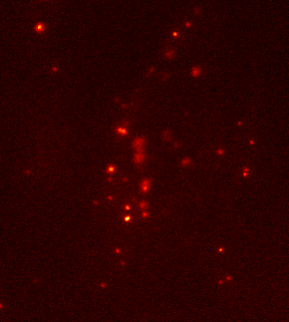
\includegraphics[width = 0.88\textwidth]{pictures/Pos2_2_red2-2frame2475Color.png}
	\caption{Raw image for dSTORM processing}
	\label{rawStorm}
\end{figure}


\section{Distributions}
\subsection{Poisson distribution}
A very important probability distribution in physics is the Poisson
distribution. Its probability mass function is:
\begin{equation}
	p(n,\mu) = \frac{\mu^n}{n!}\exp(-\mu)
\end{equation}
The larger the mean value $\mu$ gets the more likely the Poisson distribution gets to a Gaussian distribution with a mean and a variance of $\mu$. Figure \ref{poisgaussdistr} shows Poisson and Gaussian distributions with different parameters. The mean value of the gaussian was shifted by 0.5 which results from continuity correction.\newline
Poisson distributions describe the results of ``counting experiments'' and are
therefore important for image processing as pictures taken with a
camera are in principle counts of photons reaching the camera.  \newline
A Poisson distribution is defined for integer values only and its variance is
the same as the mean value of the distribution.\newline
The median of a Poisson distribution is approximatively given by
\begin{align}
	\text{median Pois}(\lambda) \approx \lambda + \frac{1}{3} - \frac{1}{50\lambda} \label{meanMedianPoiss}
\end{align}
Another important attribute is
the skewness which describes the assymetry of the distribution.
\begin{align}
 \text{skewnes Pois}(\lambda) = \frac{1}{\sqrt{\lambda}}
\end{align}
The sum of Poisson-distributed independent variables is also Poisson-distributed.
\begin{figure}
\centering
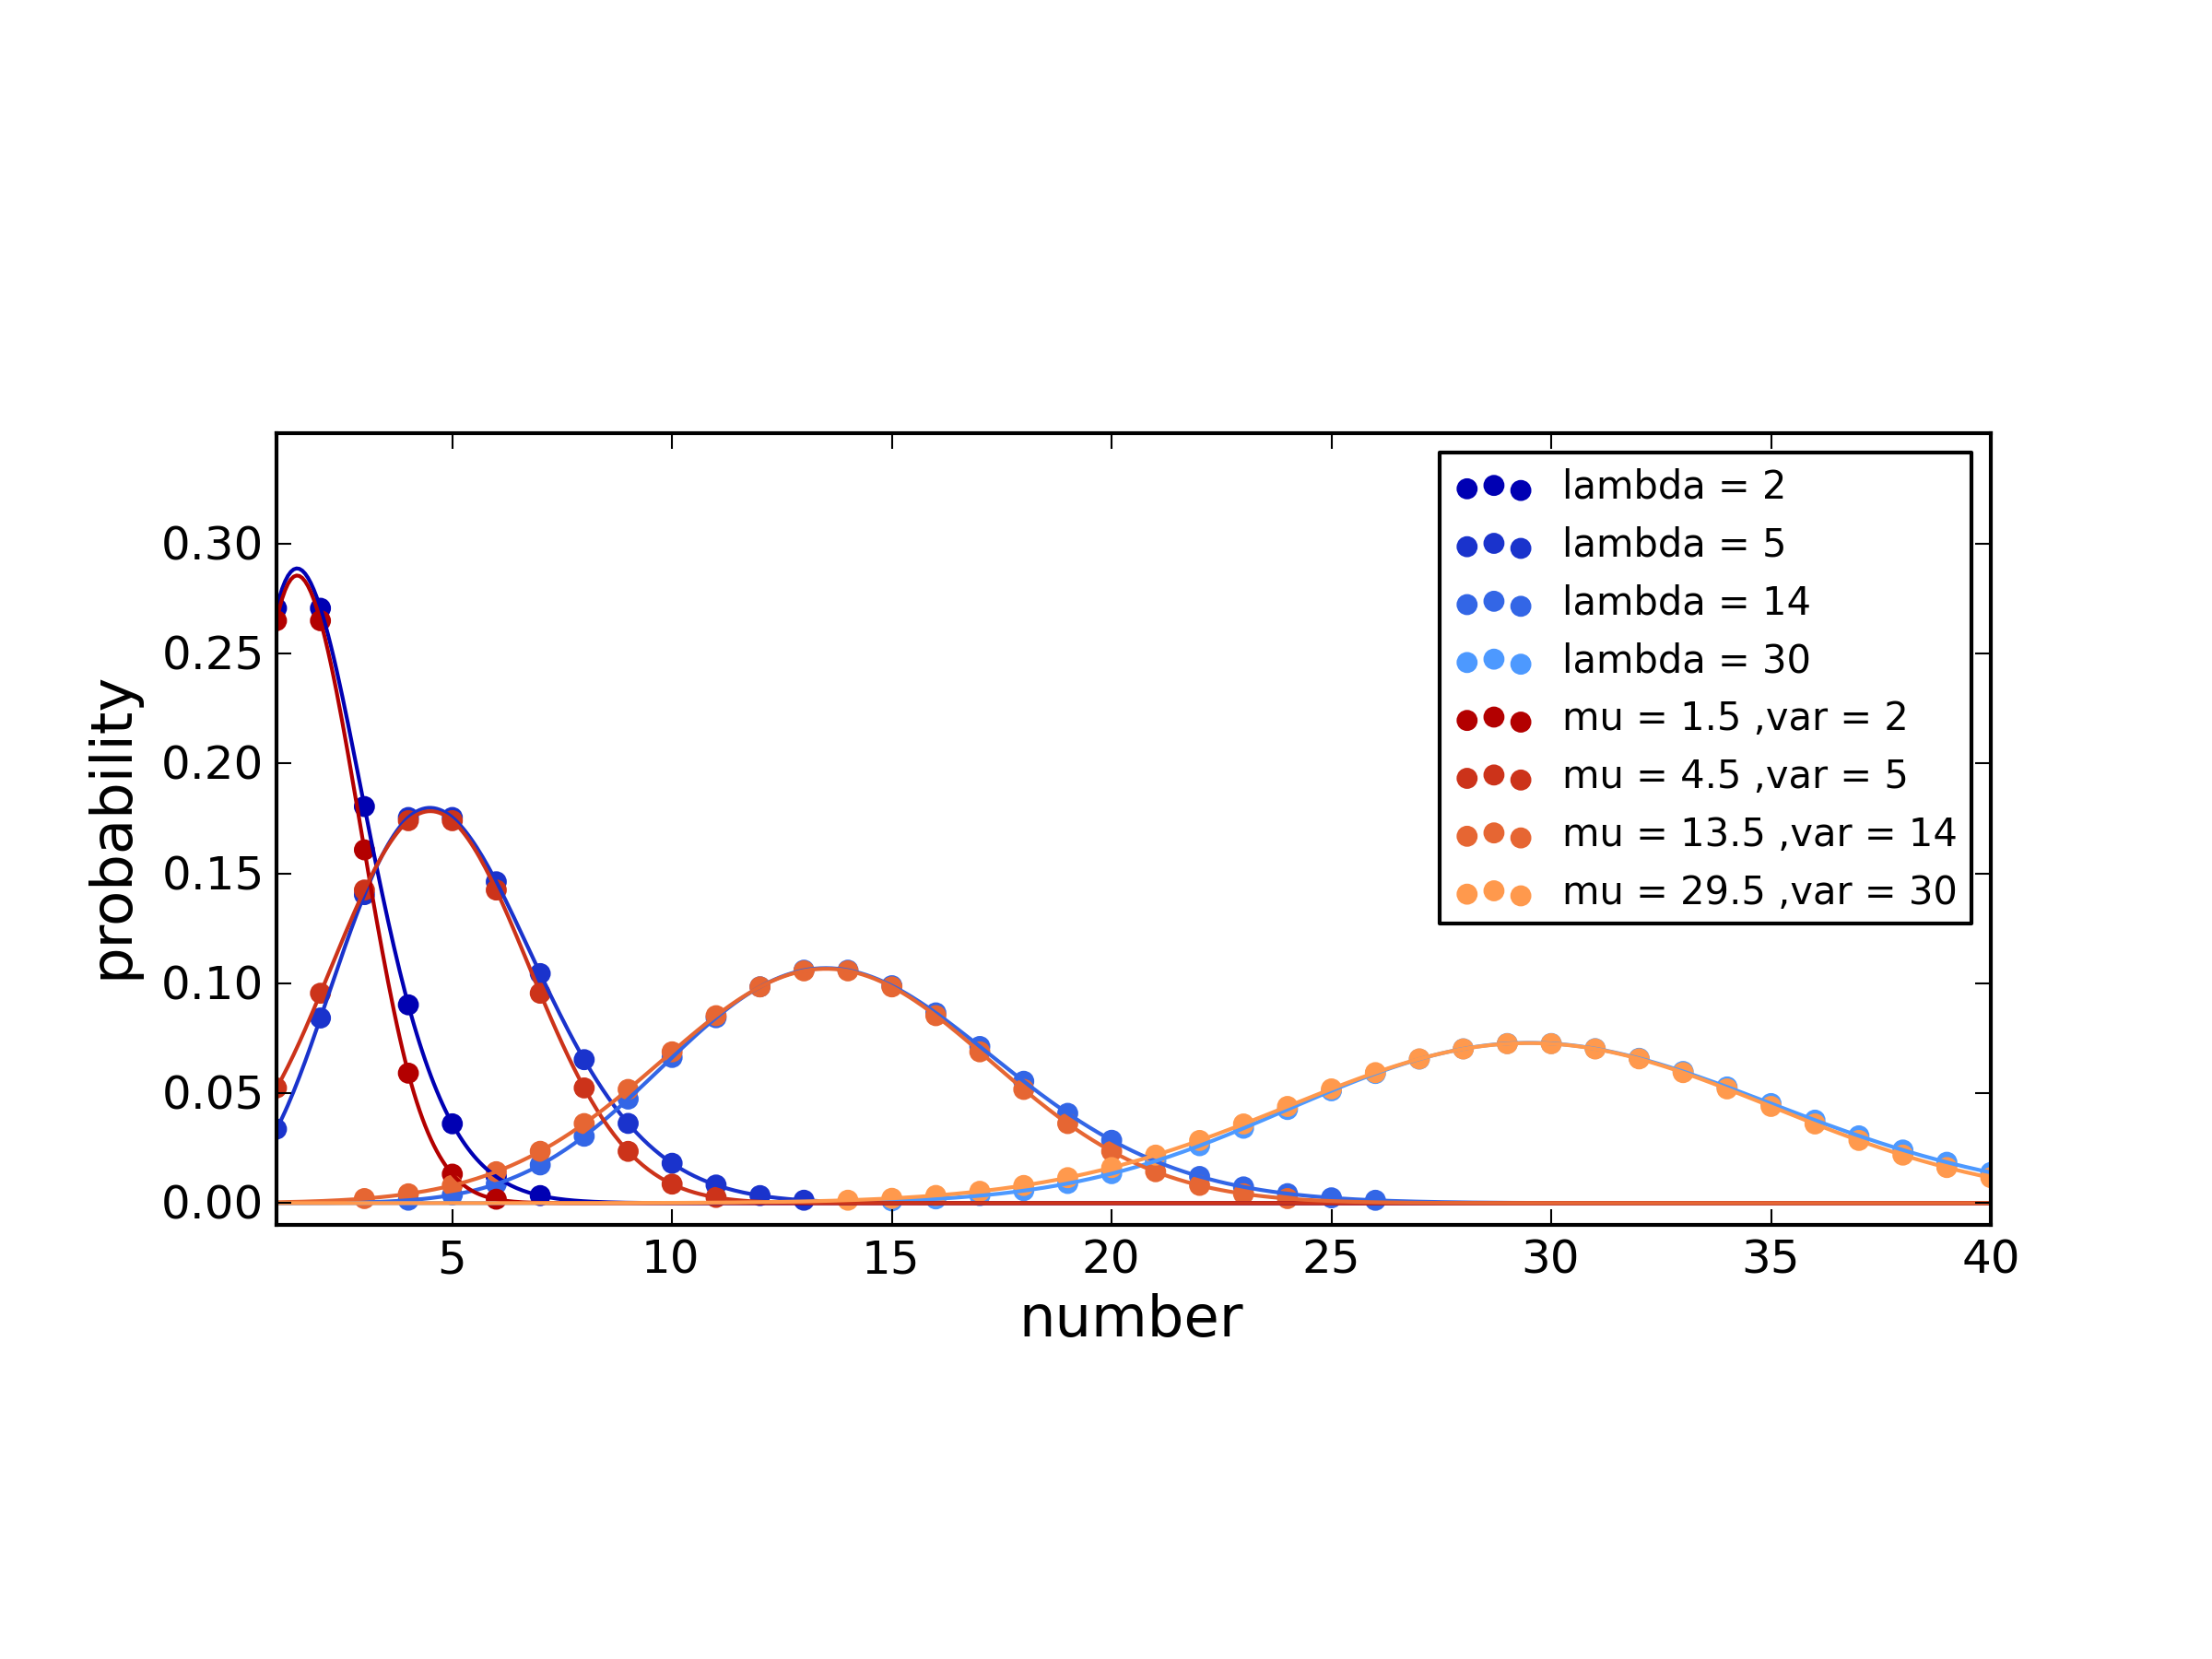
\includegraphics[width = 0.9\textwidth]{pictures/poissgaussdistr.png}
	\caption{Poisson and Gaussian distrubutions with different parameters. Especially for small numbers the Poisson and the Gaussian distribution differ. The larger $\mu$ gets for the Poisson distribution the more similar it gets to a Gaussian with mean $\mu$ and sigma $\sqrt{\mu}$. The Poisson distributions were interpolated between their defined values.}
	\label{poisgaussdistr}
\end{figure}

\subsection{Skellam distribution}
The probability
mass function of the Skellam distribution is a function of the difference between
two Poisson random variables
\begin{equation}
	p(k;\mu_1, \mu_2) =
	\exp(-(\mu_1+\mu_2))\left(\frac{\mu_1}{\mu_2}\right)^{k/2}~I_{|k|}\left(2\sqrt{\mu_1
	\mu_2}\right)
\end{equation}  
$n_1$ and $n_2$ are the Poisson distributed random variables and $k = n_1 - n_2$.
$I_{|k|}$ is the modified Bessel function of the first kind.\\
Mean $\mu$ and variance $\sigma$ of the Skellam distribution are given by
\begin{align}
	&&\mu &= \mu_1 - \mu_2,& \sigma^2 &= \mu_1 + \mu_2\\
	\Rightarrow &&\mu_1& = \frac{\mu + \sigma^2}{2},& \mu_2 &=\frac{-\mu +
	\sigma^2}{2}
\end{align}
Figure \ref{skellamdist} shows two Poisson distributions ($P_\text{red}$ and $P_\text{blue}$) and the resulting Skellam distribution (puple) of the difference $P_\text{blue} - P_\text{red}$.
\begin{figure}
\centering
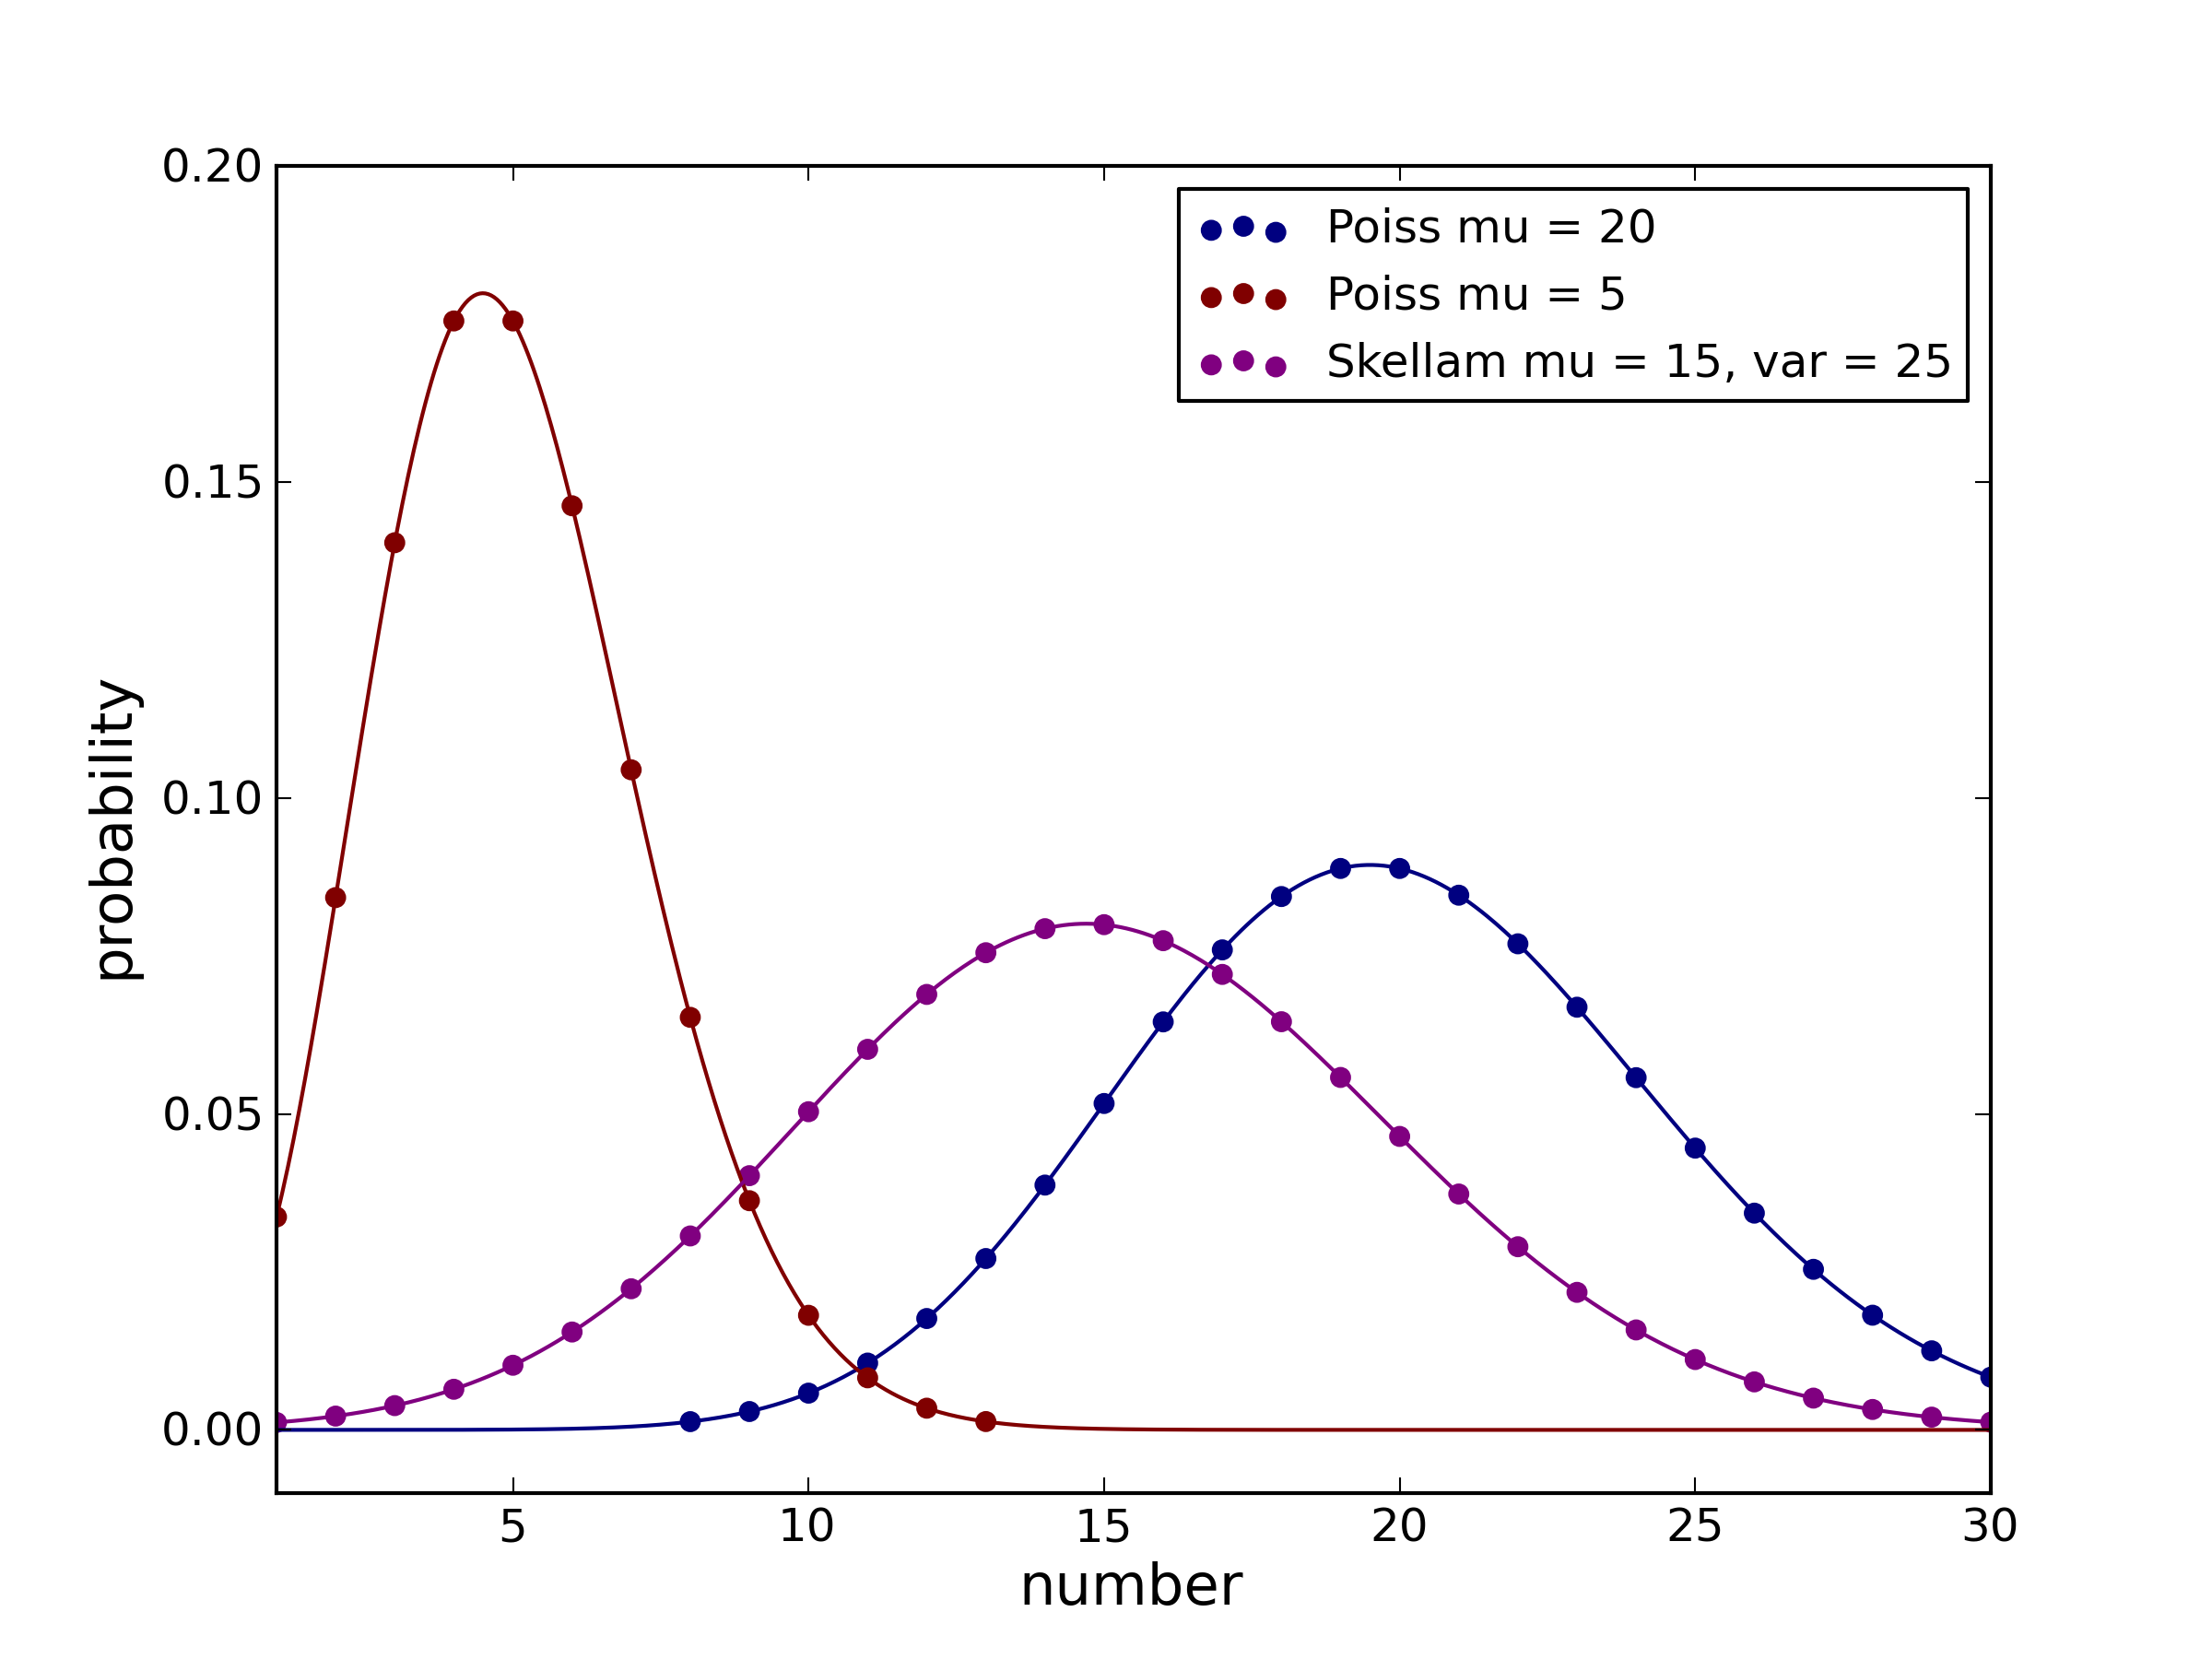
\includegraphics[width = 0.7\textwidth]{pictures/skellamdist.png}
	\caption{Two Poisson distributions and the resulting Skellam distribution. The distributions were interpolated between the integer values.}
	\label{skellamdist}
\end{figure}




\section{CCD camera}
\subsection{Photon sources with shot noise}
The emission of photons is a random process that occures at unpredictible times. Therefore the number of photons passing through a plane is never constant but varies around some average value. The phenomena, that one can never determine exactly how many photons will hit the sensor chip of a CCD camera for example, is called shot noise. It playes a major role if the total number of photons is low, as from dark sources or with short exposure times of the camera.
\subsection{Quantum efficiency}
Quantum efficiency describes the fraction of photons that creates a detectable electron in a sensor chip. The quantum efficiency dependends on the wavelenght of the incoming photon. Photons with energies below the band gap can not produce a free electron that can be detected. The quantum efficiency as a maximum for a certain wavelength. This maximum of the quantum efficiency is basically caused by two effects. The higher the energy of the photon the higher the kinetic energy of the freed electron and therefore greater diffusion length, but the electron is absorbed farer away from the detector and will therefore recombinate with a electron hole more likely.
\subsection{Gain}
There are two different gain factors involved in the capturing process of a camera. First the electric signal for each pixel might be amplified. Second there is a gain factor that describes the proportionality between collected electrons and the digital number it is associated with.
\subsection{Readout noise}
The origin of readout noise is the amplifier. The amplification is never perfect, this means that the exact number of electrons at the end of the amplification has some variation around the expected linearly increased value. There might also be some random signals of the electronics that add to the "true" signal. The readout noise does not depend on the exposure time.
\subsection{Dark current noise}
The dark current noise is generated by the thermal movement of the atoms in the sensor chip. The movement of molecules and atoms dependends on the temperature of the material, therefore dark current noise strongly depends on the temperature of the chip and can be reduced by cooling. Dark current noise generates electrons in the bins of each pixel. Even with closed shutter. It is constantly increasing with time and follows Poisson statistics.
\subsection{Quantisation}
The signal must fit into the output color depth. It has to be rounded or truncated to fit in. This process introduces errors that can be seen as additional noise that is dependent on the intensity of the signal. High intensities are disturbed less relative to low intensies.


\section{Transformations}
\subsection{Transformation to Poisson distributed signal} \label{trafoPoiss}
The images aquired from the camera do not show the real intensities
$I_\text{true}$, which result from the photon emission of the probe, but
transformed ones $I_\text{meas}$.\newline
A linearly transformation of the data is assumed with two parameters, the gain $g$ and the offset $o$.
Incoming photons create electrons via inner photoelectric effect. This electrons
are collected for each pixel and might be amplified to get the final result.
Assuming a linear relation between the number of incoming photons and the number
of electrons created and a linear amplifier results in a factor $g$. This factor
is multiplied with the number of photons captured during exposure time for each
pixel.\\
There might also be a constant offset for the pixel intensities that is not affected by the gain factor.
If the gain factor $g$ and the offset $o$ are known the true intensity, the
number of photons detected is:
\begin{equation}
	I_\text{true} = \dfrac{I_\text{meas}-o}{g}. \label{transtopoiss}
\end{equation}
After this transformation the intensities of the background are assumed to be Poisson distributed.
\subsection{Anscombe transformation}
\label{trafoAnscombe}
The Anscombe transform \cite{anscombe} is used to transform a random variable with a Poisson
distribution into one with an approximatly constant standard deviation. The
transformation is defined as:
\begin{equation}
	A(x) = 2\sqrt{x+\frac{3}{8}}.
\end{equation}
Figure \ref{anscombe} shows the standard deviation of Poisson distributions with increasing mean (green line) and the standard deviation of Poisson distributions that are transformed unsing the Anscombe transformation (blue line). As on can see in Figure \ref{anscombe} the Anscombe transformations result has
for mean intensities greater than 4 a intensity independent standard deviation of
one.
\begin{figure}
	\centering
	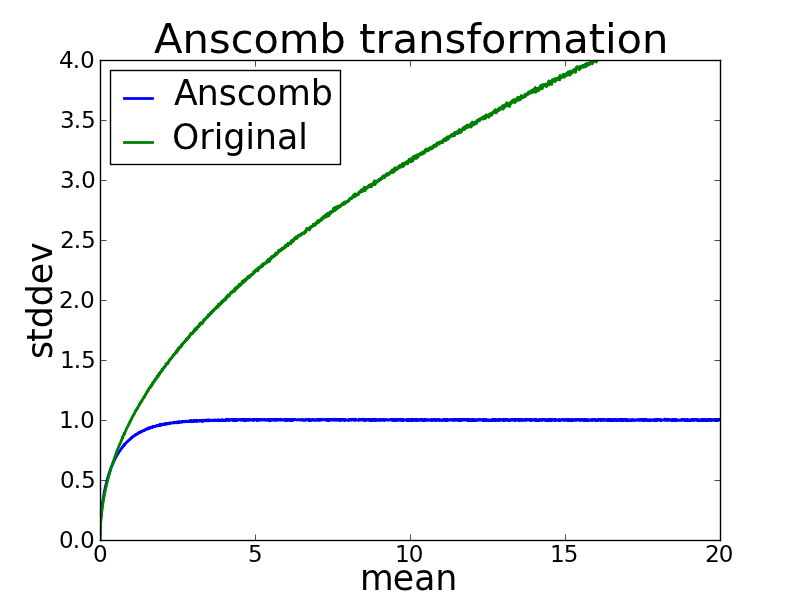
\includegraphics[width = 0.5\textwidth]{pictures/anscombe.png}
	\caption{Standard deviation over mean intensities of different Poisson
	distributions (green) and their Anscombe transformed distributions (blue)}
	\label{anscombe}
	
\end{figure}

\section{Estimation of camera gain}
Two different ways of estimating the camera parameters have been investigated. For both approaches it is assumed that the background and the beads are Poisson distributed. This data $I_\text{true}$ is then transformed in the following way:
\begin{equation}
	I_\text{meas} = g \cdot I_\text{true} + o \label{trafoGain}
\end{equation}
This is the inverse transformation of equation \ref{transtopoiss}.
\subsection{Using variance-mean plot} \label{skellam1}
The approach for the parameter estimation using the variances of the pixels is shown using a minimalistic example. It is then used in a generalised form.\newline
Considering two pixels with different Poisson distributions $P_1$ and $P_2$ with mean value and variances of this distributions $\lambda_1$ and $\lambda_2$. If this distributions are transfomed as given in equation \ref{trafoGain} their mean and variance in temporal domain change like shown in equation \ref{meanvarPoiss1} and \ref{meanvarPoiss2}. This gives the oportunity to determine the gain and offset using only two pixels.
\begin{align}
	\text{var}(I_{\text{meas}1})& = g^2\cdot\text{var}(I_{\text{true}1}) \label{calcvar}\\ 
	\text{var}(I_{\text{meas}2})& = g^2\cdot\text{var}(I_{\text{true}2})\\
	\text{mean}(I_{\text{meas}1})& = g\cdot \text{mean}(I_{\text{true}1}) + o\\
	\text{mean}(I_{\text{meas}2})& = g\cdot \text{mean}(I_{\text{true}2}) + o
\end{align}
The values for $\text{var}(I_{\text{meas}1}), \text{var}(I_{\text{meas}2})$, $\text{mean}(I_{\text{true}1})$ and $\text{mean}(I_{\text{true}2})$ can be calculated from the data and can be used to calculate the gain as follows:
\begin{align}
	\frac{\text{var}(I_{\text{meas}1})-\text{var}(I_{\text{meas}2})}{\text{mean}({\text{meas}1})-\text{mean}(I_{\text{meas}2})}&= \frac{g^2\cdot \lambda_1  - g^2\cdot \lambda_2 }{g\cdot \lambda_1 + o - (g\cdot \lambda_2+o)}\\
	& = \frac{g^2\cdot(\lambda_1-\lambda_2)}{g\cdot (\lambda_1-\lambda_2)}\\
	& = g
\end{align}
The offset $o$ can be calculated in the same way.
\begin{align}
	\text{mean}(I_{\text{meas}1}) - \frac{\text{var}(I_{\text{meas}1})}{g} &= g\cdot \lambda_1 + o - \frac{g^2\cdot\lambda_1}{g}\\
	&= o
\end{align}
The estimation gets more stable if more than two points are used and if the points are taken from a wide range of intensities. If more than two points are used a straight line must be fitted through them. The lines slope gives the gain factor and the intersection on the $x$-axis the offset. For more robustness the Skellam distribution instead of the variances is used. 
\subsection{Using skewness of poisson distribution}
A second approach is to use the skewness of the Poisson distribution to estimate the mean value.\newline
For every pixel there are multiple intensities in temporal dimension. One can
calculate mean and variance of the measured intensities for each pixel $I_\text{meas}(i,j)$ and
gets
\begin{align}
	\text{mean}(I_\text{meas}(i,j))& = g\cdot \text{mean}(I_\text{true}(i,j)) + o \label{meanvarPoiss1}\\
	\text{var}(I_\text{meas}(i,j))& = g^2\cdot\text{var}(I_\text{true}(i,j)) \label{meanvarPoiss2}
\end{align}
Assuming a Poisson distribution as the true intensity, mean and variance would
be the same. Unfortunately the mean true intensities are unknown and it is
not possible to determin $g$ and $o$ so far. For large mean Intensities $\mu$
the Poisson distribution becomes more and more symmetric and therefore similar to a Gaussian distribution
with the same mean and variance as the Poisson distribution. However, for small means, the Poisson distribution is not
symmetric. The skewness $s_p$ of a Poission distribution is the inverse of the
square root of the mean $(\mu)^{-.5}$. It can also be directly
calculated from data
\begin{equation}
	s_p = \frac{1}{n}\sum_{i = 1}^n \left(\frac{x_i - \bar x}{\sigma}\right)^3
\end{equation}
The skewness is invariant to shift and multiplication with a constant. This
means that the transformation caused by the camera gain and the offset
does not affect the skewness. This gives a third equation to solve for $g$ and
$o$.\\
This approach is strictly limited to, at least for background pixels, low intensities. Tests have shown that if the mean of the true Poisson distribution is higher than roughly 30, the skewness gives, due to noise, no stabel results. For data sets with bright background intensities it is not possible to determine the camera parameters in this way.

\section{Chromatic aberration}
In microscopy it is often desirable to label different structures in a cell with
different colors. To do so our collaborators use different fluoroscent molecules
that emit light at different and therefore distinguishable wavelengths. Using appropriate
filters it is possible to capture pictures just containing light emited from one
kind of fluorophore.\newline
The propagation speed of light depends on the substance it is propagating through. The property of the substance that describes the ratio of the speed of light in vacuum $c$ and in the substance $v$ is called refraction index $n = c/v$.\newline
The refraction index for one substance is wavelength dependent. Different wavelengths are refrected under different angles. This effect causes the splitting of white light into its components when shining through a prism.\newline
The same effect causes the focal length of the microscope to be wavelength dependent. This means that the light for the same spot but with
different wavelenghts is not mapped to the same spot in the image. This is shown in Figure \ref{wikibild1}.

\begin{figure}
	\centering
	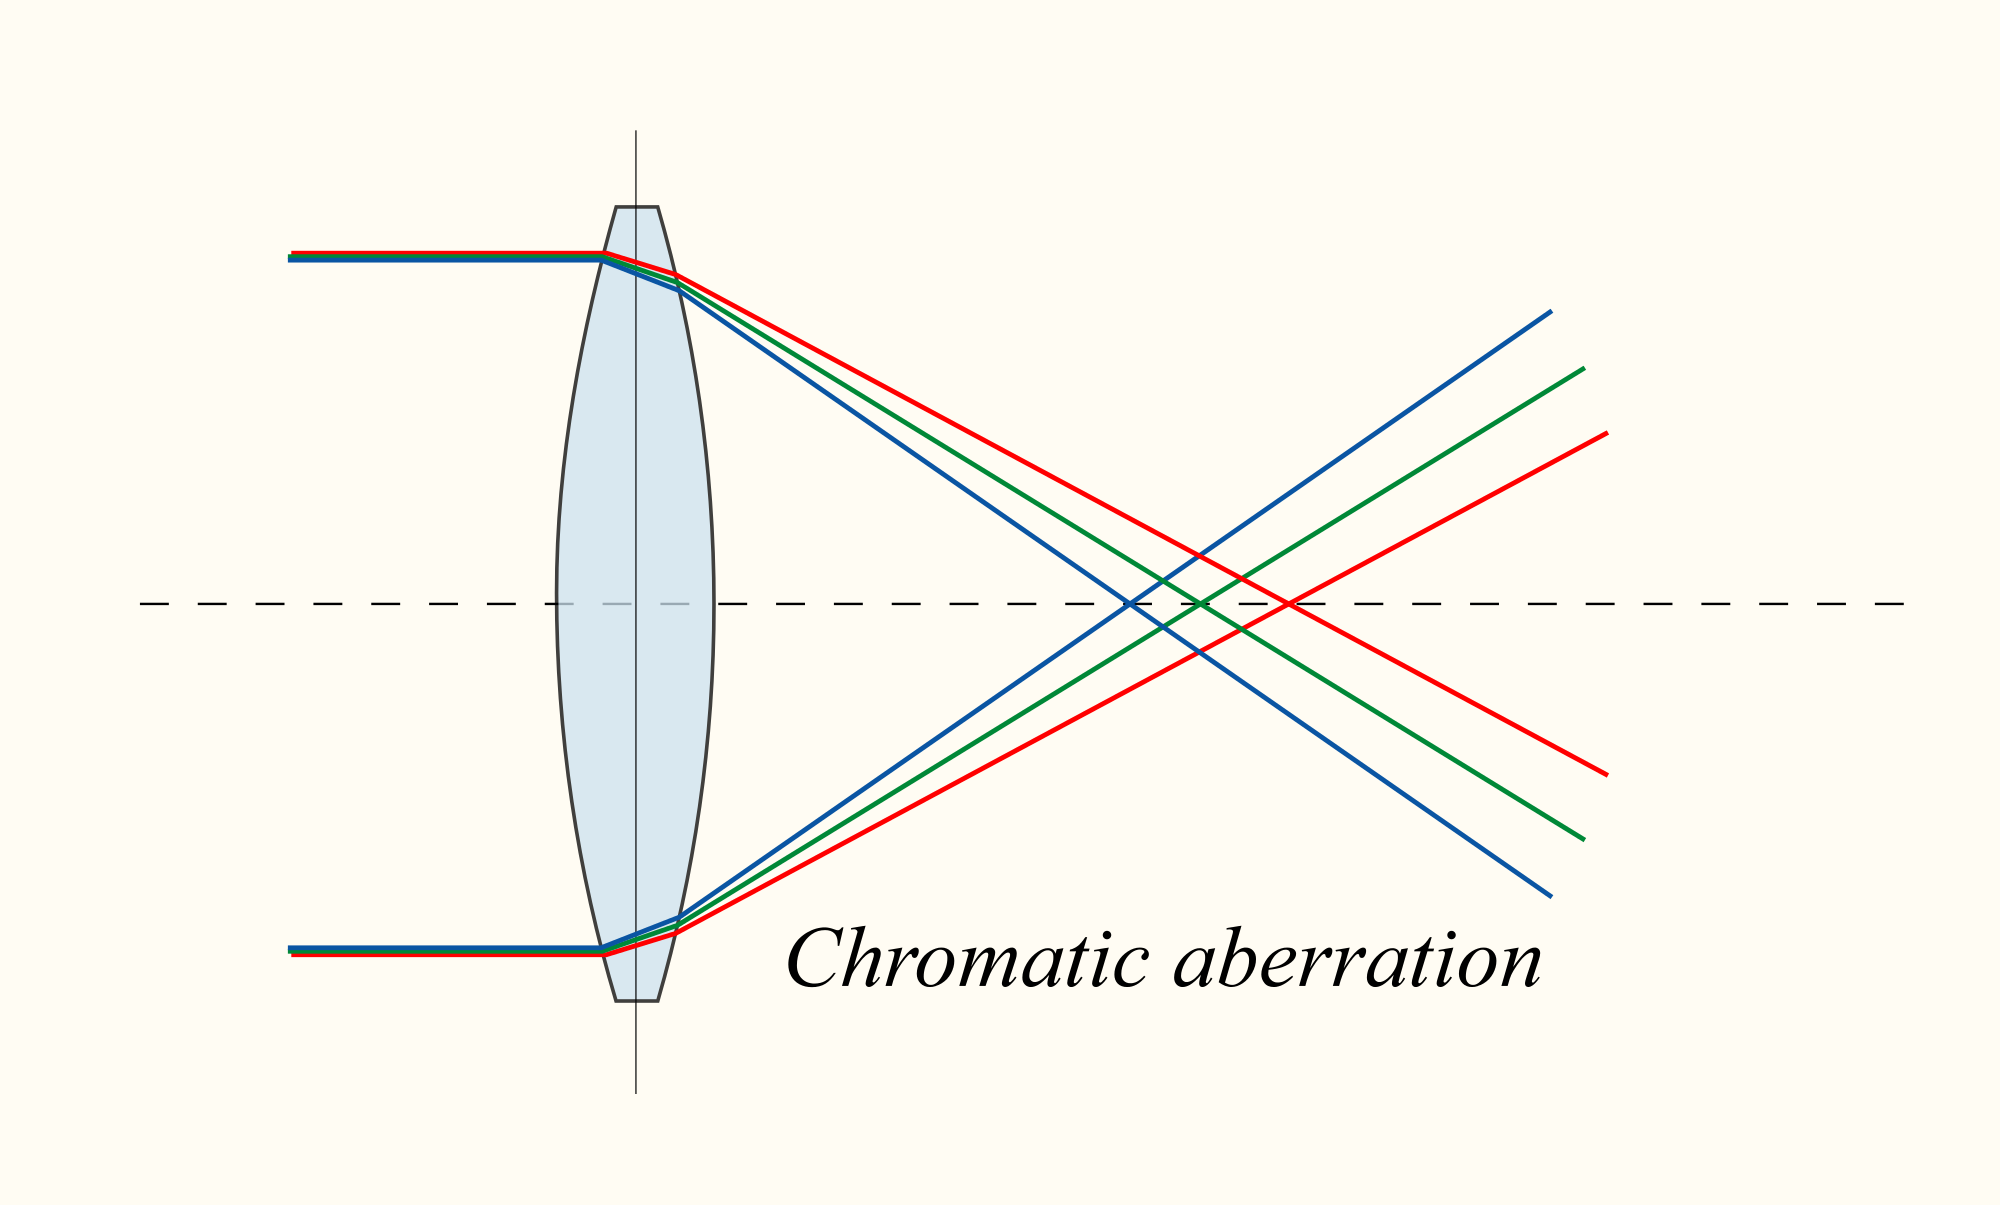
\includegraphics[width = 0.5\textwidth]{pictures/bildabberationwiki.png}
	\caption[Chromatic aberration, picture taken from http://en.wikipedia.org/wiki /File:Chromatic\_abberation\_lens\_diagram.svg, at 23rd of May 2013]{Sketch of the dependency of the focal length on the wavelength.}
	\label{wikibild1}
	\end{figure}
